\item \points{6d}

Complete the function \texttt{log\_likelihood} in \texttt{src/submission/likelihood.py} to compute the log-likelihoods for each string. 
The histograms of the log-likelihoods of strings for each file should look like those in Fig. \ref{fig:ll}.

\begin{figure}
    \centering
    \begin{subfigure}{0.3\textwidth}
        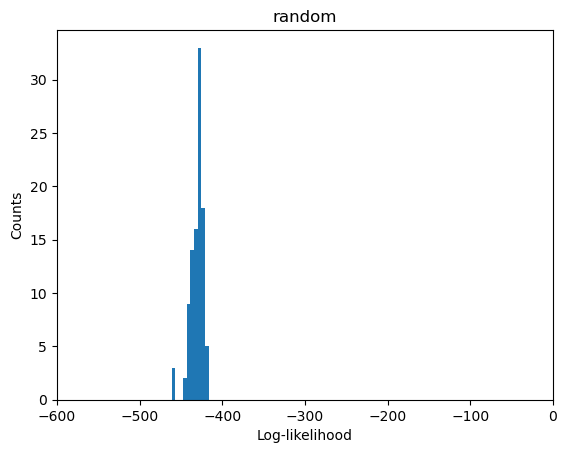
\includegraphics[width=\linewidth]{./figures/random}
    \end{subfigure}
    \begin{subfigure}{0.3\textwidth}
        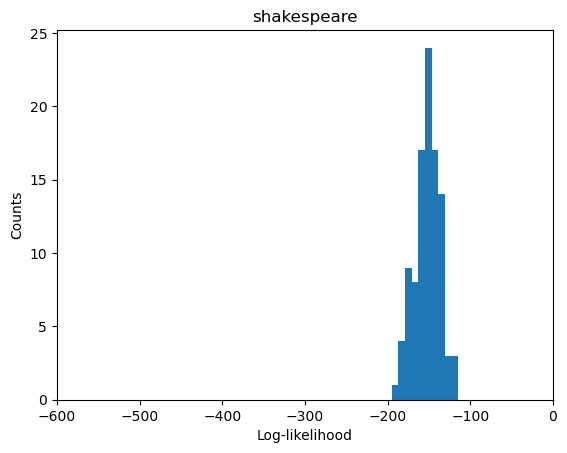
\includegraphics[width=\linewidth]{./figures/shakespeare}
    \end{subfigure}
    \begin{subfigure}{0.3\textwidth}
        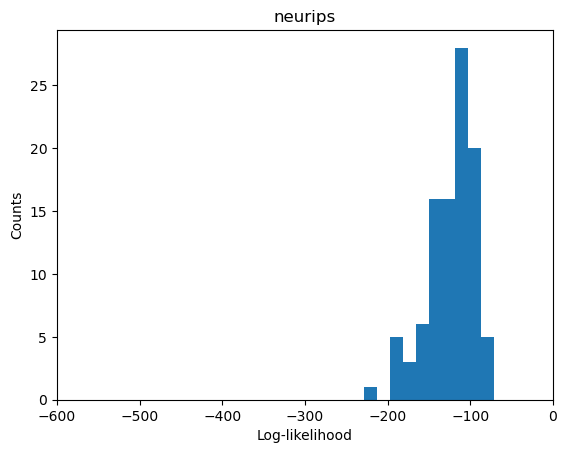
\includegraphics[width=\linewidth]{./figures/neurips}
    \end{subfigure}
    \caption{Expected log likelihood histograms for each text type}
    \label{fig:ll}
\end{figure}